\chapter{\leavevmode\newline Example Chapter Title}
\label{chap:chapter_2}


%% main text

\section{Introduction}
This chapter will show you how to include figures, references, equations, and tables in your thesis. Figure \ref{FIG: engine and num model diagram} is show below. Another figure (Fig. \ref{FIG: Two figs}) is also shown which include two figures together. This is how you cite a source \cite{yang2019bee+} \cite{nellis_klein_2012}. 


\begin{figure*}
\centering
  \makebox[\textwidth][c]{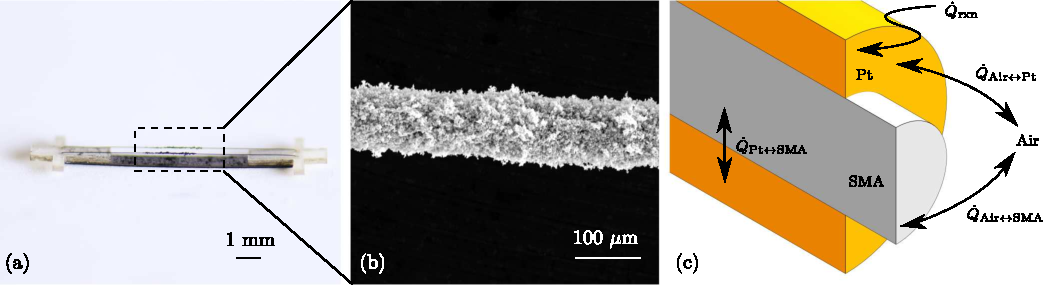
\includegraphics[width=1\textwidth]{figures/fig_1.pdf}}
        \caption{Example Figure.}
        \label{FIG: engine and num model diagram}
\end{figure*}


\begin{figure}
\centering
\begin{subfigure}{.49\textwidth}
  \centering
  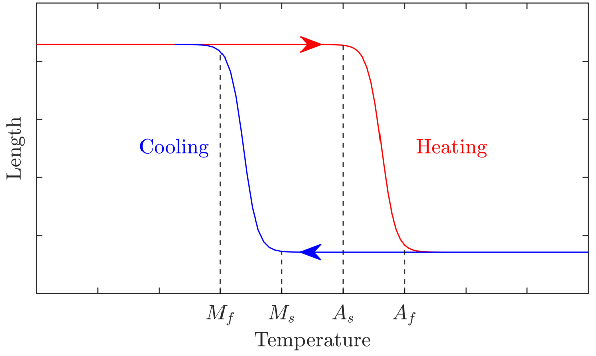
\includegraphics[width=1\linewidth]{figures/fig_2.pdf}
  \caption{Hydrogen in propane}
  \label{fig:sub1}
\end{subfigure}
\begin{subfigure}{.49\textwidth}
  \centering
  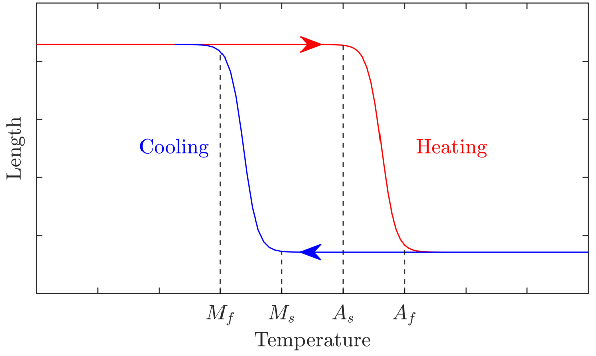
\includegraphics[width=1\linewidth]{figures/fig_2.pdf}
  \caption{Hydrogen in nitrogen}
  \label{fig:sub2}
\end{subfigure}
\caption{Example of two figures together}
\label{FIG: Two figs}
\end{figure}



An equation (Eq. \ref{eq: Biot Definition})is shown below:
\begin{equation}
B_i = \frac{L_{\text{cond}}\bar{h}}{k}
\label{eq: Biot Definition}
\end{equation}

\subsection{Example Subsection and tables}

This is an example of a subsection. This is a table:


\begin{table}[t] \centering
\begin{tabular}{@{}lc@{}}
\toprule
System and Dimension       & ${B_{i}}$ \\ \midrule
SMA Radial       & 7.2    \\
SMA Longitudinal  & 0.38    \\
Pt Radial         & 1.6    \\
Pt Longitudinal  & 0.21    \\ \bottomrule
\end{tabular}
\caption{{Biot Number for the radial and longitudinal dimensions in the system.}}
\label{tab:Biot Summary}
\end{table}


